\documentclass[10pt,letterpaper]{article}
\usepackage[latin1]{inputenc}
\usepackage[spanish]{babel}
\usepackage{amsmath}
\usepackage{amsfonts}
\usepackage{amssymb}
\usepackage{graphicx}
\usepackage{fancyhdr}
%\usepackage[uft8]{inputenc}
\usepackage[left=4cm,right=3cm,top=4cm,bottom=3cm]{geometry}
\author{Maycol Gonzalez-Gerardo Carvajal}
\title{Documentacion Arbol-B}


\begin{document}
\maketitle
\newpage
\tableofcontents
\newpage
%***********************************************************************************
\section{Descripcion Arbol-B}
\vskip 0.5cm
Los arboles b disenados para funcionar bien en discos u otros accesos directos
dispositivos de almacenamiento secundario.Los arboles B son similares a los arboles red-black, pero son mejores para minimizar las operaciones de E / S de disco. Muchos sistemas de bases de datos utilizan B-trees, o variantes de B-trees, para almacenar informacion.
\vskip 0.3cm
La idea tras los arboles-B es que los nodos internos deben tener un numero variable de nodos hijo dentro de un rango predefinido. Cuando se inserta o se elimina un dato de la estructura, la cantidad de nodos hijo varía dentro de un nodo. Para que siga manteniendose el numero de nodos dentro del rango predefinido, los nodos internos se juntan o se parten. Dado que se permite un rango variable de nodos hijo, los arboles-B no necesitan Re balancearse tan frecuentemente como los arboles binarios de busqueda auto-balanceables. Pero, por otro lado, pueden desperdiciar memoria, porque los nodos no permanecen totalmente ocupados.
\vskip 2cm
%**********************************************************************************
\section{Caracteristicas Arbol-B}
\vskip 0.3cm
Los Arboles B deben cumplir las sigientes caracteristicas:
\vskip 0.3cm
\begin{itemize}
\item Toda pagina tiene como maximo 2n nodos.
\item Toda pagina distinta de la raiz tiene como minimo n nodos.
\item La raiz tiene como minimo un nodo.
\item Todas las paginas hojas estan en el ultimo nivel.
\end{itemize}
\vskip 0.3cm
Ademas de estas caracteristicas los arboles B tienen cumplir cierto orden:
\vskip 0.3cm
\begin{itemize}
\item Los nodos dentro de una pagina mantienen un orden ascendente.
\item Cada nodo es mayor que los nodos situados a su izquerda.
\item Cada nodo es mayor que los nodos situados a su derecha.
\end{itemize}
\vskip 0.3cm
\newpage
%***********************************************************************************
\section{Implementacion Arbol-B}
\vskip 0.3cm
En esta seccion, presentamos los detalles de algunas de las operaciones basicas del los arboles B como los es crear,Buscar, eliminar e Insertar:
\vskip 0.3cm
%***********************************************************************
\begin{itemize}
\item Crear Arbol B: Para construir un T arbol B, primero usamos B-TREE-CREATE para crear un nodo raiz vacio y luego agregamos nuevas claves.
\vskip 0.3cm
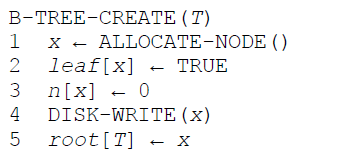
\includegraphics[width=5cm,height=3cm]{crear} 
\vskip 0.3cm

%**************************************************************
\skip 0.3cm

\item Buscar: Buscar un arbol B es muy parecido a buscar en un arbol binario de busqueda, excepto que en lugar de hacer un
decision de bifurcacion binaria o "bidireccional" en cada nodo, hacemos una bifurcacion de multiples vias
decision segun el numero de hijos del nodo.

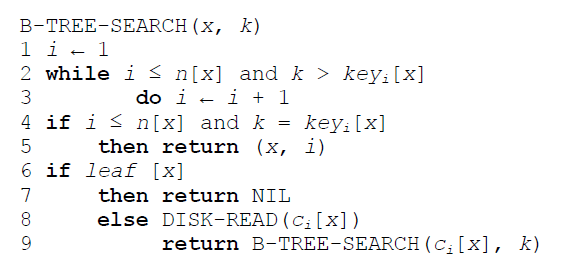
\includegraphics[width=10cm,height=5cm]{buscar} 
\vskip 0.3cm
Usando un procedimiento de busqueda lineal, las lineas 1-3 encuentran el indice mas pequeno i tal que k <= key i (x), o
de lo contrario, establecen i a n [x] + 1. Las lineas 4-5 comprueban si ahora hemos descubierto la clave, volviendo
si tenemos Las lineas 6-9 terminan la busqueda sin exito (si x es una hoja)  en el
busque el subarbol apropiado de x, despues de realizar el DISK-READ necesario en ese hijo
%*********************************************************************
\vskip 5cm
\item Insertar: Las inserciones se hacen en los nodos hoja.\\
\begin{itemize}
 \item 1. Realizando una busqueda en el arbol, se halla el nodo hoja en el cual deberia ubicarse el nuevo elemento.
 \item 2. Si el nodo hoja tiene menos elementos que el maximo numero de elementos legales, entonces hay lugar para uno mas. Inserte el nuevo elemento en el nodo, respetando el orden de los elementos.\\
 \item 3. De otra forma, el nodo debe ser dividido en dos nodos. La division se realiza de la siguiente manera:
 \begin{itemize}
 
 \item Se escoge el valor medio entre los elementos del nodo y el nuevo elemento.
 \item Los valores menores que el valor medio se colocan en el nuevo nodo izquierdo, y los valores mayores que el valor medio se colocan en el nuevo nodo derecho; el valor medio actua como valor separador.
 \item El valor separador se debe colocar en el nodo padre, lo que puede provocar que el padre sea dividido en dos, y asi sucesivamente.

 \end{itemize}
\end{itemize}
\vskip 0.4cm
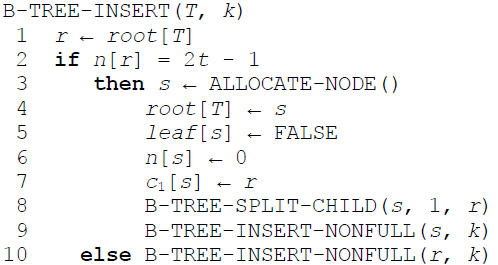
\includegraphics[width=8cm,height=5cm]{inserta}{ Insercion normal}
\vskip 0.3cm
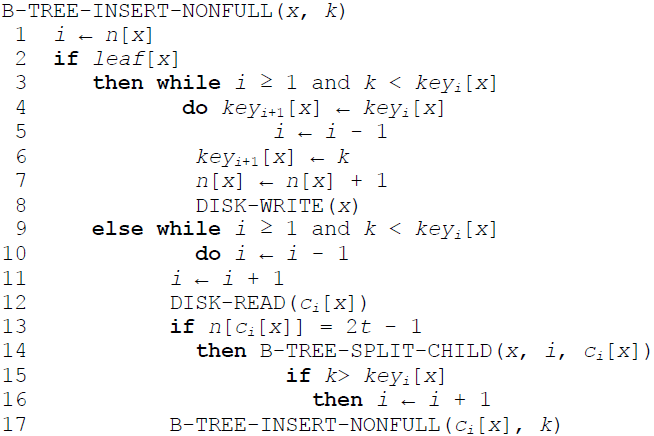
\includegraphics[width=9cm,height=7cm]{inserta2}{ Insercion con divicion de nodo}
\vskip 0.9cm

\item Eliminar:La eliminacion de un B-tree es analoga a la insercion, pero un poco mas complicada, porque una clave
puede eliminarse de cualquier nodo, no solo una hoja, y la eliminacion de un nodo interno requiere que
los hijos del nodo se reorganizen. Al igual que en la insercion, debemos protegernos contra la eliminacion produciendo un
arbol cuya estructura viola las propiedades del arbol B. Asi como tunemos que asegurarnos de que un nodo no
se hace demasiado grande debido a la insercion, debemos asegurarnos de que un nodo no se vuelva demasiado pequeno durante la eliminacion
(excepto que la raiz tiene permitido tener menos que el numero minimo t - 1 de teclas, aunque no esta permitido tener mas que el numero maximo 2t - 1 de teclas).


\end{itemize}
\newpage
\section{Referencias}
\begin{itemize}
\vskip 0.8cm
\item Libro CLRS.
\end{itemize}

\end{document}\documentclass[11pt]{article}

